\documentclass[a4paper]{article}
\usepackage[utf8]{inputenc}
\usepackage[T2A]{fontenc}
\usepackage[english, russian]{babel}
\usepackage[warn]{mathtext}
\usepackage{graphicx, placeins, tabularx}
\usepackage{amsmath}
\usepackage{floatflt}
\usepackage[left=20mm, top=20mm, right=20mm, bottom=20mm, footskip=10mm]{geometry}


\graphicspath{ {images/} }
\usepackage{multicol}
\setlength{\columnsep}{2cm}


\title{Лабораторная работа 3.3.4:\\Эффект Холла в полупроводниках}
\author{Дроздов Т. А.\\Кириллов М. А.\\Б03-202}
\date{}

\begin{document}
\maketitle

\textbf{В работе используются}: электромагнит с источником питания GPR, батарейка 1,5 В, амперметр, реостат, цифровой вольтметр B7-78/1, милливеберметр, образцы легированного германия.


\section*{Выполнение работы}


    Проведём калибровку электромагнита - исследуем зависимость индукции магнитного поля в зазоре электромагнита от тока через обмотки магнита. Для этого определим поток Ф вектора магнитной индукции, который пронизывал пробную катушку, находившуюся в зазоре ($\Phi = BSN$) для различных значений тока через электромагнит. Результаты занесём в таблицу 1.
    
    % \begin{table}[h]
    % \centering
    % \begin{center}
    % \caption{Калибровка электромагнита}
    % \end{center}
    % \vspace{0.1cm}
    % \label{tab:my_label}
    % \begin{tabular}{ |p{1.5cm}||p{0.7cm}|p{0.7cm}|p{0.7cm}|p{0.7cm}|p{0.7cm}|p{0.7cm}|p{0.7cm}|p{0.7cm}|  }
%  \hline
% $I_M, A$ & 0 & 0.3 & 0.6 & 0.9 & 1.2 & 1.5 & 1.8 & 2.08 \\
%  \hline
%  $\Phi, $мВб & 0.15 & 1.7 & 3.3 & 4.9 & 6.25 & 7.2 & 7.8 & 8.3\\
%  \hline
%  $B, $Тл & 0.021 & 0.236 & 0.458 & 0.681 & 0.868 & 1.000 & 1.083 & 1.153\\
%  \hline

\begin{table}[]
\begin{tabular}{|l|r|r|r|r|r|r|r|r|r|r|}
\hline
I, A     & 0.20 & 0.40 & 0.60 & 0.80 & 1.00 & 1.20 & 1.40 & 1.60 & 1.80 & 1.92 \\ \hline
Phi, mWb & 0.95 & 1.90 & 2.80 & 3.65 & 4.50 & 5.20 & 5.75 & 6.20 & 6.55 & 6.80 \\ \hline
B, Tl    & 0.13 & 0.25 & 0.37 & 0.49 & 0.60 & 0.69 & 0.77 & 0.83 & 0.87 & 0.91 \\ \hline
\end{tabular}
\end{table}

\FloatBarrier

    \begin{figure}[h]
    \centering
    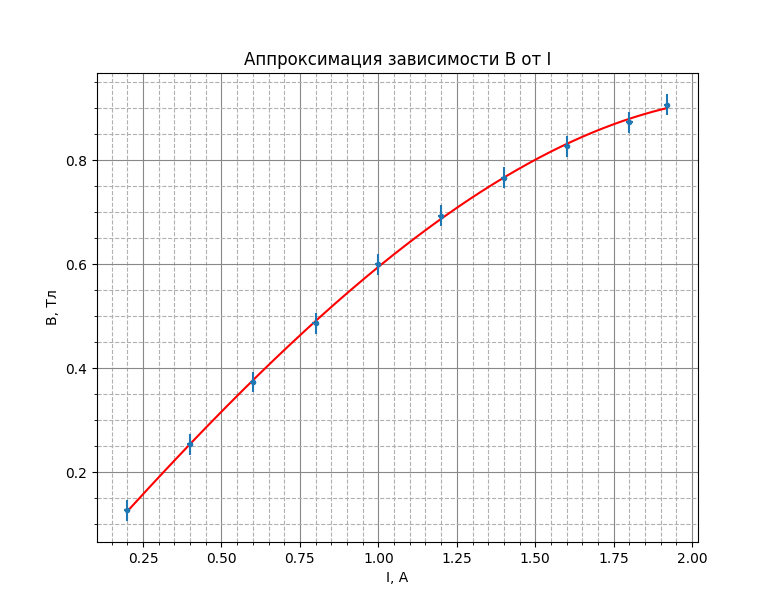
\includegraphics[width=15cm]{curve.png}
    \caption{График калибровки электромагнита}
    \label{fig:cal}
\end{figure}

\FloatBarrier
    
     Проведём измерение ЭДС Холла. Снимем зависимость напряжения $U_{34}$ от тока $I_M$ через обмотки магнита при фиксированно токе через образец. Выполним серию экспериментов для различных токов через образец $I$ (от 0.3 до 1 мА). Результаты измерений занесём в таблицу 2.
    
%     \begin{table}[h]
%     \centering
%     \begin{center}
%     \caption{Зависимость напряжения в образце от тока в обмотке электромагнита}
%     \end{center}
%     \vspace{0.1cm}
%     \label{tab:hall-dependency}
%     \begin{tabular}{ |p{3cm}||p{0.7cm}|p{0.7cm}|p{0.7cm}|p{0.7cm}|p{0.7cm}|p{0.7cm}|p{0.7cm}|p{0.7cm}|p{0.7cm}|p{0.7cm}|p{0.7cm}|  }
%  \hline
% $I_M, мA$ & 0 & 0.21 & 0.42 & 0.63 & 0.84 & 1.05 & 1.26 & 1.47 & 1.68 & 1.89 & 2.06\\
%  \hline
%  $B, $Тл & 0.000 & 0.184 & 0.352 & 0.506 & 0.645 & 0.769 & 0.878 & 0.973 & 1.052 & 1.116 & 1.157\\
%  \hline
%  \hline
% $U_{34}, B (I = 0.3$мА) & 0.069 & 0.088 & 0.107 & 0.126 & 0.142 & 0.156 & 0.169 & 0.177 & 0.184 & 0.189 & 0.192\\
% \hline
% $U_{34}, B (I = 0.4$мА) & 0.092 & 0.116 & 0.143 & 0.167 & 0.189 & 0.208 & 0.225 & 0.236 & 0.245 & 0.251 & 0.255\\
% \hline
% $U_{34}, B (I = 0.5$мА) & 0.115 & 0.146 & 0.178 & 0.209 & 0.237 & 0.26 & 0.281 & 0.295 & 0.305 & 0.301 & 0.319\\
% \hline
% $U_{34}, B (I = 0.6$мА) & 0.139 & 0.175 & 0.215 & 0.254 & 0.285 & 0.313 & 0.338 & 0.356 & 0.368 & 0.378 & 0.383\\
% \hline
% $U_{34}, B (I = 0.7$мА) & 0.161 & 0.205 & 0.25 & 0.293 & 0.332 & 0.366 & 0.394 & 0.415 & 0.429 & 0.441  &  \\
% \hline
% $U_{34}, B (I = 0.8$мА) & 0.184 & 0.233 & 0.286 & 0.335 & 0.38 & 0.416 & 0.449 & 0.473 & 0.483 & 0.502 & 0.509\\
% \hline
% $U_{34}, B (I = 1.0$мА) & 0.231 & 0.292 & 0.358 & 0.418 & 0.457 & 0.521 & 0.563 & 0.591 & 0.613 & 0.629 & 0.635\\
% \hline
% \hline

%  \end{tabular}
% \end{table}

\begin{table}[]
\begin{tabular}{|r|r|r|r|r|r|r|r|r|r|r|r|}
\hline
\multicolumn{1}{|l|}{I, mA \textbackslash I\_em, A} & 0.00  & 0.20  & 0.40  & 0.60  & 0.80  & 1.00  & 1.20  & 1.40  & 1.60  & 1.80  & 2.00  \\ \hline
0.30                                                & -0.01 & -0.03 & -0.05 & -0.07 & -0.09 & -0.10 & -0.12 & -0.13 & -0.14 & -0.15 & -0.15 \\ \hline
0.40                                                & -0.02 & -0.05 & -0.07 & -0.10 & -0.12 & -0.14 & -0.16 & -0.18 & -0.19 & -0.20 & -0.21 \\ \hline
0.50                                                & -0.03 & -0.06 & -0.09 & -0.12 & -0.15 & -0.18 & -0.20 & -0.23 & -0.24 & -0.25 & -0.26 \\ \hline
0.60                                                & -0.04 & -0.07 & -0.11 & -0.15 & -0.18 & -0.21 & -0.25 & -0.27 & -0.29 & -0.30 & -0.31 \\ \hline
0.70                                                & -0.04 & -0.09 & -0.13 & -0.17 & -0.22 & -0.25 & -0.29 & -0.32 & -0.33 & -0.35 & -0.36 \\ \hline
0.80                                                & -0.05 & -0.10 & -0.15 & -0.20 & -0.25 & -0.29 & -0.33 & -0.36 & -0.38 & -0.40 & -0.42 \\ \hline
0.90                                                & -0.06 & -0.11 & -0.17 & -0.22 & -0.28 & -0.33 & -0.37 & -0.41 & -0.43 & -0.45 & -0.47 \\ \hline
1.00                                                & -0.07 & -0.13 & -0.19 & -0.25 & -0.31 & -0.36 & -0.41 & -0.45 & -0.48 & -0.50 & -0.52 \\ \hline
-1.00                                               & -0.07 & -0.01 & 0.06  & 0.12  & 0.17  & 0.22  & 0.27  & 0.31  & 0.33  & 0.35  & 0.37  \\ \hline
\end{tabular}
\end{table}

\begin{figure}[h]
    \centering
    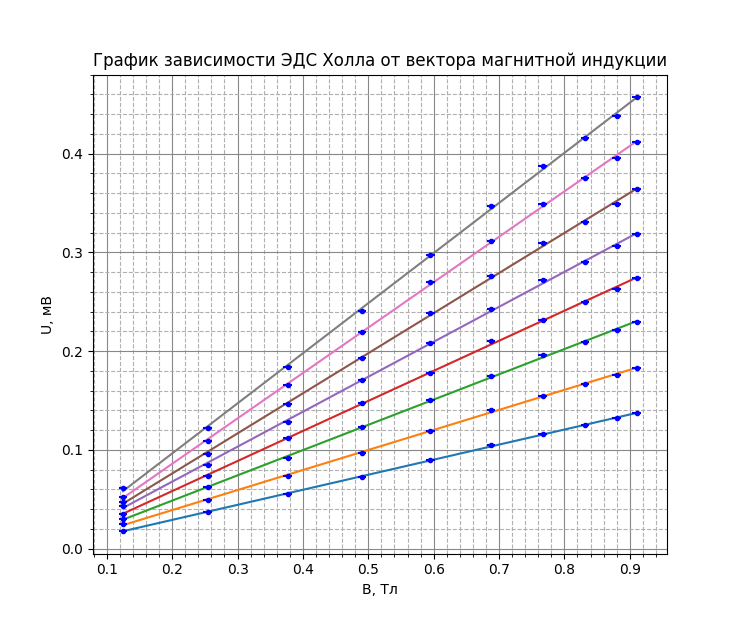
\includegraphics[width=\textwidth]{hall-dependency.png}
    \caption{Семейство зависимостей ЭДС Холла от магнитного воля в электромагните при разных токах через образец}
    \label{fig:vac}
\end{figure}
\par

\FloatBarrier

\begin{figure}[h]
    \centering
    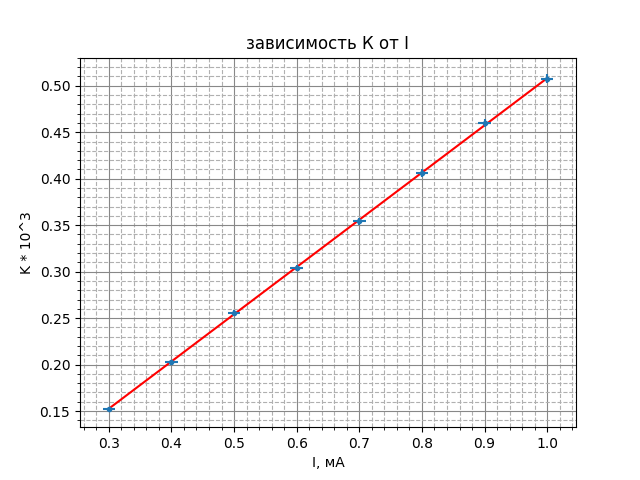
\includegraphics[width=15cm]{k-dependency.png}
    \caption{Определение постоянной Холла}
    \label{fig:k-dep}
\end{figure}

\FloatBarrier

Определив угловые коэффициенты прямых (рис.2), построим график зависимости $K = f(I)$ (рис. 3). Рассчитаем угловые коэффициенты $K(I) = \Delta E / \Delta B$ и определим величину постоянной Холла $R_x$. Погрешность рассчитаем по методу наименьших квадратов, учитывая погрешности приборов.



\begin{center}
  $R_x = - k a = (7.62 \pm 1.10)10^{-4} $ м$^3$/Кл  
\end{center}

Относительная погрешность составляет 8,6\%.

Учитывая рис. 4, направление тока в образце и знак ЭДС Холла, определим характер проводимости в образце по правилу векторного произведения. Проводимость дырочная.

\begin{figure}
    \centering
    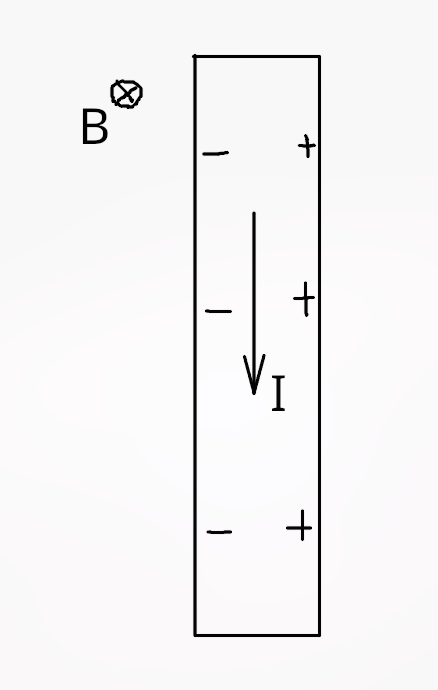
\includegraphics[width=0.5\linewidth]{image.png}
    \caption{образец с электронной проводимостью в магнитном поле}
    \label{fig:enter-label}
\end{figure}

\FloatBarrier
Рассчитаем концентрацию носителей тока:

\begin{center}
    $n = \frac{1}{R_x e} = (8.2 \pm 0.18)10^{21}$ед/м$^3$
\end{center}

По формуле (3) рассчитаем удельную проводимость исследуемого образца. При $I = 1$ мА $U_{35} = 2.16 $В, параметры установки: $a = 2.2mm, l = 7 mm, L_{35} = 6 mm$
 \begin{center}
     $\sigma = 668.4 \pm 6.7$ 1/(Ом м)
 \end{center}
 
 Наконец, рассчитаем подвижность носителей в образце.
 \begin{center}
     $b = \frac{\sigma}{ne} = 5095 \pm 120 $см$^2$/(В*с) \\
     $b_{theor} = 3800$ см$^2$/(В*с) для электронной проводимости
 \end{center}


\section*{Вывод}

В ходе работы был исследован эффект Холла в полупроводнике-германии. Были определены такие характеристики, как постоянная Холла, концентрация холловских частиц, удельная электрическая проводимость германия и подвижность электронов-носителей заряда в нём. Результаты совпали с табличными по порядку величины. Возможная причина несовпадения - характер проводимости в исследуемом образце не чисто электронный, а электронно-дырочный (подвижность носителей заряда уменьшится). \\
Был проведён небольшой опрос среди студентов, выполнявших эту работу. Выяснилось, что на одной установке (у окна) полученное значение подвижности электронов сходилось с табличным, а на другой (ближе к двери) - была меньше практически на 2000 единиц. Самое разумное объяснение этого - то, что исследуемый образец не является чистым германием, а лигированным, с иными свойствами. Даже мельчайшие доли примесей способны изменять подвижность носителей заряда на тысячи единиц.


\end{document}